\section{Introduction}
\label{sec:intro}
Nowadays, advent of consumer friendly and affordable depth-cameras such as Kinect are commercially employed in many applications such as robotics and virtual reality.
%
Understanding and interpreting raw data provided by depth-cameras has drawn many attentions of researchers.
%
Whilst semantic segmentation as a fundamental part for understanding these raw data develops rapidly.
%
In the field of semantic segmentation, indoor scene parsing is a challenging problem due to cluttered backgrounds, a wide rang of scenes, object occlusions and various illumination.

\begin{figure}[htbp]
	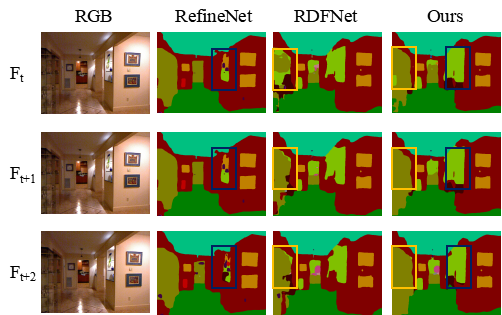
\includegraphics[scale=0.65]{figure/Consist.png}
	\vspace*{-0.6cm} 
	\caption{An illustration of “jumping” problem. The  prediction results by deffierent methods of adjacent frames are shown and some details are framed.}
	\label{fig:Consist}
	\vspace*{-0.35cm}
\end{figure}


In recent years, a great deal of studies have been conducted can be divided into three groups.
%
One group conducted semantic segmentation from single RGB image.
%
Another one attempted to add auxiliary information from depth for better segmentation results.
%
The last one is multi-task learning which learns semantic segmentation with other tasks at the same time.


{\bf Semantic Segmentation from Single Image.}
%
Fully convolutional network (FCN) ~\cite{Long2015} is a milstone-like work for pixel-wise segmentation that converted the existing CNN constructed for classification to semantic segmentation.
%
To overcome the limitations of FCN that the network limited by a pre-defined fixed-size receptive field and always lost the detailed structures of objects, Noh \emph{et al.} \cite{Noh2015} proposed a novel deconvolution algorithm. 
%
Bayesian SegNet \cite{Kendall2015} performed visual scene understanding with a measure of model uncertainty to produce a probabilistic segmentation result.
%
To capture semantic correlations between neighboring patches and expoit the
patch-patch contextual information, Lin \emph{et al.} \cite{Lin2016} formulated conditional random fields (CRFs) with CNN-based pairwise potential function. 
%
For generating fine prediction, Lin \emph{et al.} \cite{Lin2017} proposed a multi-path refinement network that effectively exploits multi-level features to refine the prediction step by step.
%
Semantic segmentation from a single image often leads to incomplete segmentation results. 
%
As the predictions from RefineNet \cite{Lin2017} shown in Fig.~\ref{fig:Consist}.

\begin{figure*}[htbp]
	\vspace{-0.6cm}
	\setlength{\abovecaptionskip}{0pt} 
	\setlength{\belowcaptionskip}{10pt}
	\centering
	\centering
	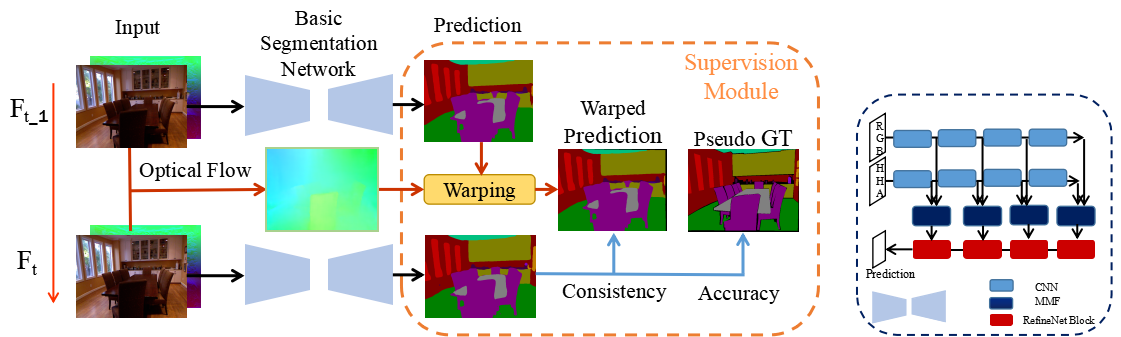
\includegraphics[scale=0.57]{figure/Pipeline.png}
	\vspace*{-0.8cm} 
	\caption{The diagram of our proposed methods. The left one is pseudo ground truth propagation. We propagate the GT from labeled frame to their adjacent frames by image warpping. The right one is flow chart of training segmentation network using temporal consistncy. It mainly consists of three steps: 1) The current frame $F_t$ passes through a basic semantic segmentation network to generate the prediction  2) Warpping the prediction of previous frame $F_{t-1}$ depends on optical flow generated from PWC-Net \cite{Sun2018} 3) Warpped prediction of $F_{t-1}$ and generated PGT joint action on the network by $L_{consistency}$ and $L_{PGT}$ respectively.}
	\label{fig:Pipeline}
	\vspace*{-0.2cm}
\end{figure*}

{\bf Semantic Segmentation with Depth.}
%
Using extracted features from RGB images and depth data, Gupta \emph{et al.} \cite{Gupta2014} implemented an integrated system for scene understanding.
%
 A novel long short-term memorized context fusion (LSTM-CF) model is propposed by Li \emph{et al.} \cite{Li2016} to fuse contextual information from multiple sources such as RGB images and depth data.
% 
Cheng \emph{et al.} \cite{Cheng2017} rethought the relationship between RGB images and depth, and proposed a locality-sensitive deconvolution network to refine the boundary of segmentation result as well as a gated fusion layer to combine features of two modes.
%
Park \emph{et al.} \cite{Park2017} worked on how to fuse the multi-level RGB-D CNN features.
%
Therefore, they proposed a multi-modal feature fusion blocks and added it to RefineNet \cite{Lin2017}.
%
Although adding depth information improves the performance of single image segmentation, the predictions between consecutive frames are jumped due to the temporal relationship is not taken into account.
%
Fig.~\ref{fig:Consist} shows the "jumping" problem.

{\bf Multi-task Learning.} 
%
Eigen and Fergus \cite{Eigen2015} addressed three different tasks such as depth prediction, surface normal estimation, and semantic labeling using a single multiscale convolutional netwrok. 
%
Prediction-and-distillationn network (PAD-Net) is another work\cite{Xu2018} which predicts a set of intermediate tasks including depth, surface normal, semantic and contour estimation, and then using the predictions from these tasks as multi-modal disitillation modules' inputs for final tasks.  
%
A novel joint Task-Recursive Learning (TRL) \cite{Zhang2018} framework for semantic segmentation and depth estimation was proposed by Zhang. 
%
In TRL, two tasks are alternately processed in the decoder to imporve each other.
% 
Jiao \emph{et al.} \cite{Jiao2018} presented an attention-driven loss for network supervision and a synergy network to learn the information sharing strategies. 
%
By combining two tasks as well as proposed attention-driven loss, the performance of depth estimation and semantic segmentation are mutuallty improved.
%
Although the multi-task learning method improves the segmentation results, it needs supplementary information or even data from other tasks, and the overall process is more complex.

Above approaches provide a lot of novel ideas to improve the segmentation results, but the ability and performance of these methods are greatly limited by the limited dense-annotated training data.
%
Meanwhile, dense-annontated data is expensive to obtain.
%
In order to take full use of a large quantity of non-annotated data, in this paper, we propose two simple but effective approaches. 
%
One is propagating labels from annotated frame to neighbouring non-aonnotated frames that generates many good quality and mixed noise pseudo ground truth (PGT) for network training. 
%
Compared to common data augmentation operations, it increases the diversity of training data.
%
The other is proposing a training policy that training a semantic segmentation network with a temporal consistency constraint between frames. 
%
The rest of this paper is organized as follows.
% 
Our methodology will be introduced firstly.
%
Then, we will report the extensive experimental results as well as analyses. 
%
Finally we will draw a conclusion and propose our future work.
